\subsubsection{Captura activa}

En este caso tenemos un comportamiento similar al descrito previamente, esto es para $\phi > p_v + 2(D_i -1) p_d$ tenemos que $f$ decae exponencialmente a partir de un valor de $k_{ij}$ \emph{suficientemente grande}, y a su vez crece exponencialmente para valores \emph{suficientemente peque\~nos}, dado que $f \in C^1$ esto a su vez nos dice que debe existir un punto m\'aximo para $f$ sin embargo en este caso no tenemos una expresi\'on an\'alitica para $k^*$ salvo que cumple la siguiente relaci\'on:

\begin{equation}
  (k^*)^{\phi}((k^*)^{2p_v}(p_v+ h -\phi) + (h -\phi) + (k^*)^{2p_v - \phi}(p_v + h ) ) + h = 0
\end{equation}

Con $h$ igual que en el caso $grazing$.\\
De esta relaci\'on podemos obtener que :
\begin{equation}
  k^*_{Active} \in ] k^*_{Grazing} , k^*_{Sit} [
\end{equation}

A su vez para $\phi \leq 2(D_i - 1)p_d $ podemos esperar un crecimiento mon\'otono por parte de $f$. 

\begin{figure}
\begin{center}
 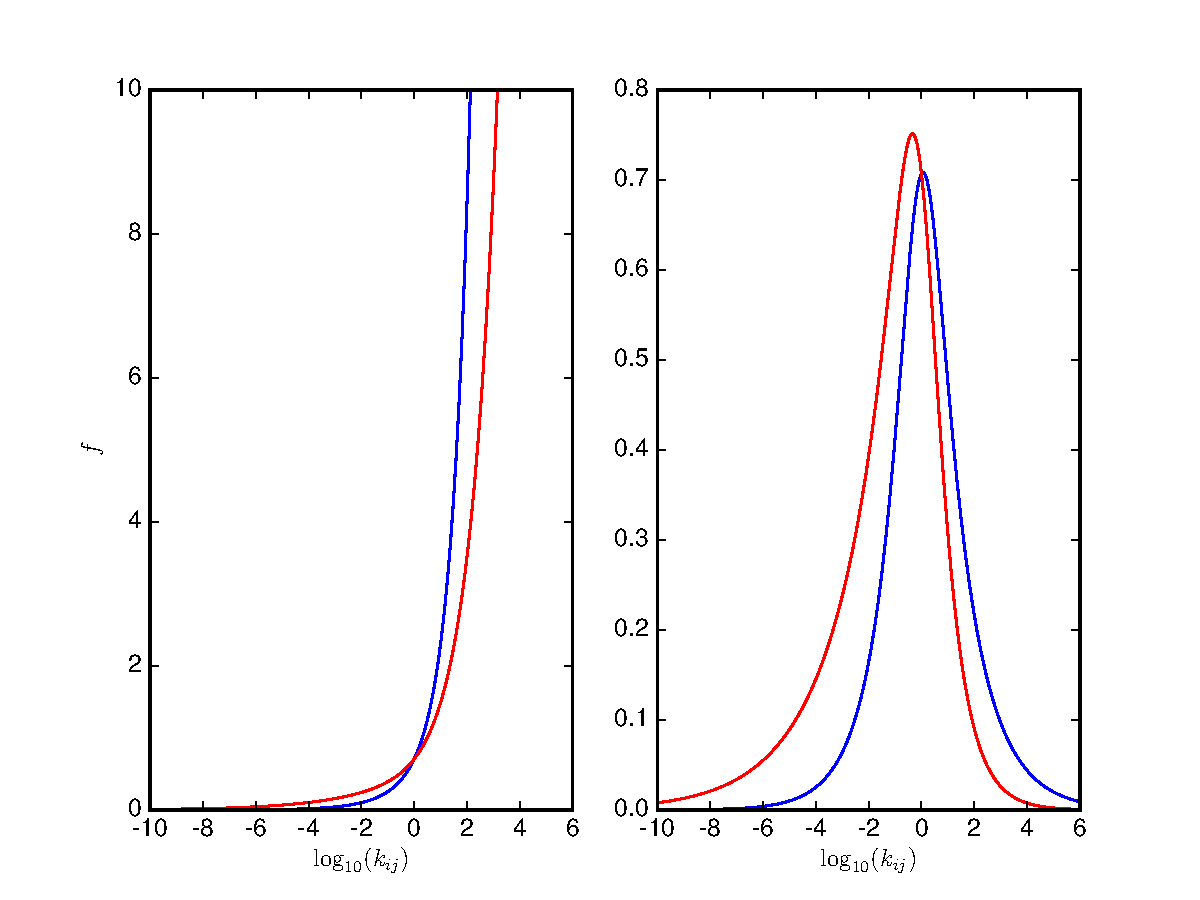
\includegraphics[width=0.9\textwidth]{./Plots/f1Active.pdf}
 \caption[$f_1, Active$]{$f$ en funci\'on a $k_{ij}$, con $a =1$, para el caso de una estrategia de forrajeo \emph{activa}, las dem\'as especificaciones se comparten con la figura \ref{fig:f1Grazing}}
 \label{fig:f1Active} 
\end{center}
\end{figure}

